\section{Problema de la 3-Coloración (3C)}

% ------------------------------------------------------------------------------\
% -----------------------------------------------------------------------------\
\subsection{\textcolor{Contraste4}{Forma Canónica}}
% ------------------------------------------------------------------------------\
% -----------------------------------------------------------------------------\

\begin{myitemize}

    \item \textbf{Problema} 
    
    Dada una grafica $(G = (V, E))$ ¿Es posible asignar un color a cada vértice de manera que ningún 
    par de vértices adyacentes comparta el mismo color, utilizando un máximo de tres colores?
    
    \item \textbf{Entrada}
    
    Un gráfica no dirigida $( G = (V, E) )$, donde $(V)$ es el conjunto de vértices y $(E)$ es el 
    conjunto de aristas.

    \item \textbf{Pregunta}
    
    ¿Es posible colorear cada vértice de $G$ tal que ningún par de vértices adyacentes compartan el mismo color?
\end{myitemize}

% ------------------------------------------------------------------------------\
% -----------------------------------------------------------------------------\
\subsection{\textcolor{Contraste4}{Demostrar que el problema esta en NP}}

\subsubsection*{\textcolor{Contraste3}{Algoritmo No-determinístico P}}
% ------------------------------------------------------------------------------\
% -----------------------------------------------------------------------------\

\begin{verbatim}
entrada = Un grafica G=(V,E)

Inicio
1. Aleatoriamente asignar un color (de los 3 disponibles) 
    a cada vertice de G
2. Verificamos la asignación
    para cada par de vértices adyacente
    a) Si u y v tienen el mismo color
        rechazar la asignación.
    b) Si no se rechazó en el paso anterior
        aceptar la asignación.

3. Si se encuentra una asignación válida, aceptar; 
    de lo contrario, rechazar.
FIN
\end{verbatim}

El algoritmo no determinista se ejecuta en tiempo polinomial porque sería la suma de los 
tiempos de ejecución de cada paso $O(|V| + |E|)$: La asignación de colores se puede 
realizar en tiempo $O(|V|)$, donde $|V|$ es la cantidad de vértices en la gráfica y la
verificación se puede realizar en tiempo $O(|E|)$ donde $|E|$ son el total de aristas
recorridas en toda la ejecución.\\ 

Esto quiere decir que como el algoritmo puede asignar aleatoriamente los colores y verificar 
la asignación, si existe una asignación valida de 3 colores para una grafica tal que dos 
vértices adyacentes no estan del mismo color significa que logramos encontrar una solución. 

%Si: Supongamos que I tiene una solución con 3 colores. Entonces, existe una asignación de colores c:V→{1,2,3} tal que no hay dos vértices adyacentes con el mismo color. El algoritmo no determinista puede adivinar esta asignación y luego verificarla en tiempo polinomial. Por lo tanto, el algoritmo no determinista aceptará I.

%Solo si: Supongamos que el algoritmo no determinista acepta I. Entonces, existe una asignación de colores c:V→{1,2,3} que el algoritmo no determinista verifica. Esta asignación no tiene dos vértices adyacentes con el mismo color. Por lo tanto, I tiene una solución con 3 colores.

% ------------------------------------------------------------------------------\
% -----------------------------------------------------------------------------\
\subsection{\textcolor{Contraste4}{Demostrar transformación}}
% ------------------------------------------------------------------------------\
% -----------------------------------------------------------------------------\

\subsubsection*{\textcolor{Contraste3}{Problema de Satisfacción Booleana (SAT)}}

Dada una expresión booleana $E$ compuesta por variables booleanas $x_{1}, x_{2},. . .,x_{n}$
y cláusulas booleanas $C_{1}, C_{2},. . .,C_{m}$, el problema SAT busca determinar si existe 
una asignación de verdad a las variables que haga que la expresión $E$ sea verdadera.

\subsubsection*{\textcolor{Contraste3}{Problema de la 3-coloración}}

Dada una gráfica $G = (V,E)$, el problema de la 3-coloración busca determinar si es posible asignar 
un color a cada vértice de $G$ de manera que ningún par de vértices adyacentes comparta el mismo 
color, utilizando un máximo de tres colores..


\begin{enumerate}
    \item Descripción de la Transformación
    
    Dada una instancia de 3SAT con variables $x_{1}, x_{2}, \ldots, x_{n}$ y cláusulas $C_1, C_2, \ldots, C_m$, 
    construimos un gráfico ( G ) de la siguiente manera:
    \begin{myitemize}
        \item Para cada variable $x_i$, creamos un vértice para $x_i$ y un vértice para su negación $\bar{x}_i$.
        \item Conectamos cada par de vértices $x_i$ y $\bar{x}_i$ con una arista, ya que no pueden tener el mismo 
                valor de verdad (color).
        \item Para cada cláusula $C_j$, creamos un triángulo de cláusula conectando tres vértices que representan 
                los literales de la cláusula.
        \item Conectamos cada vértice del triángulo de cláusula con los vértices correspondientes de las variables 
                o sus negaciones.
    \end{myitemize}

    \item Demostración de la Equivalencia
    
    \begin{myitemize}
        \item Si 3SAT es satisfactorio: Si tenemos una asignación de verdad que satisface todas las cláusulas, 
                asignamos colores de la siguiente manera:
        \begin{myitemize}
            \item Si $x_i$ es verdadero, coloreamos el vértice $x_i$ con color 1 y $\bar{x}_i$ con color 2.
            \item Si $x_i$ es falso, hacemos lo contrario.
            \item Cada triángulo de cláusula puede ser coloreado con tres colores ya que al menos uno de sus 
                    vértices tendrá un color diferente debido a la asignación de verdad satisfactoria.
        \end{myitemize}
        \item Si G puede ser coloreado con tres colores: La asignación de colores a los vértices de las variables 
                nos da una asignación de verdad para 3SAT:
        \begin{myitemize}
            \item Si el vértice $x_i$ tiene color 1, asignamos verdadero a $x_i$, si tiene color 2, asignamos falso.
            \item Como los triángulos de cláusula están coloreados correctamente, al menos uno de los literales 
                    de cada cláusula debe ser verdadero, satisfaciendo así la instancia de 3SAT.
        \end{myitemize}
    \end{myitemize}    
\end{enumerate}

La clave de esta transformación es que una coloración válida de la gráfica $G$ corresponderá a una asignación 
de verdad que satisface todas las cláusulas de $E$, y viceversa. Por lo tanto, esta transformación permite 
utilizar los algoritmos existentes para resolver el problema de la 3-coloración para determinar la satisfacibilidad
de la expresión booleana $E$


% ------------------------------------------------------------------------------\
% -----------------------------------------------------------------------------\
\subsection{\textcolor{Contraste4}{Ejemplificar}}
% ------------------------------------------------------------------------------\
% -----------------------------------------------------------------------------\

\subsubsection*{\textcolor{Contraste3}{Transformación a 3-Coloración}}

Instancia de 3SAT: Supongamos que tenemos la siguiente expresión booleana con tres cláusulas:
\begin{equation*}
    (x_1 \vee \bar{x}_2 \vee x_3) \wedge (x_2 \vee \bar{x}_3 \vee x_4) \wedge (\bar{x}_1 \vee x_2 \vee  \bar{x}_4)
\end{equation*}

\begin{enumerate}
    \item Variables
    \begin{myitemize}
        \item Para cada variable $x_i$, creamos dos vértices: uno para $x_i$ y otro para $\bar{x}_i$.
        \item Conectamos cada par de vértices correspondientes a una variable y su negación con una arista.
    \end{myitemize}

    \item Cláusulas
    \begin{myitemize}
        \item Para cada cláusula, creamos un triángulo de cláusula conectando tres vértices que 
                representan los literales de la cláusula.
    \end{myitemize}

    \item Conexiones
    \begin{myitemize}
        \item Conectamos los vértices de las variables a los vértices correspondientes en los triángulos 
                de cláusula según su aparición en las cláusulas.
    \end{myitemize}

    \begin{center}
        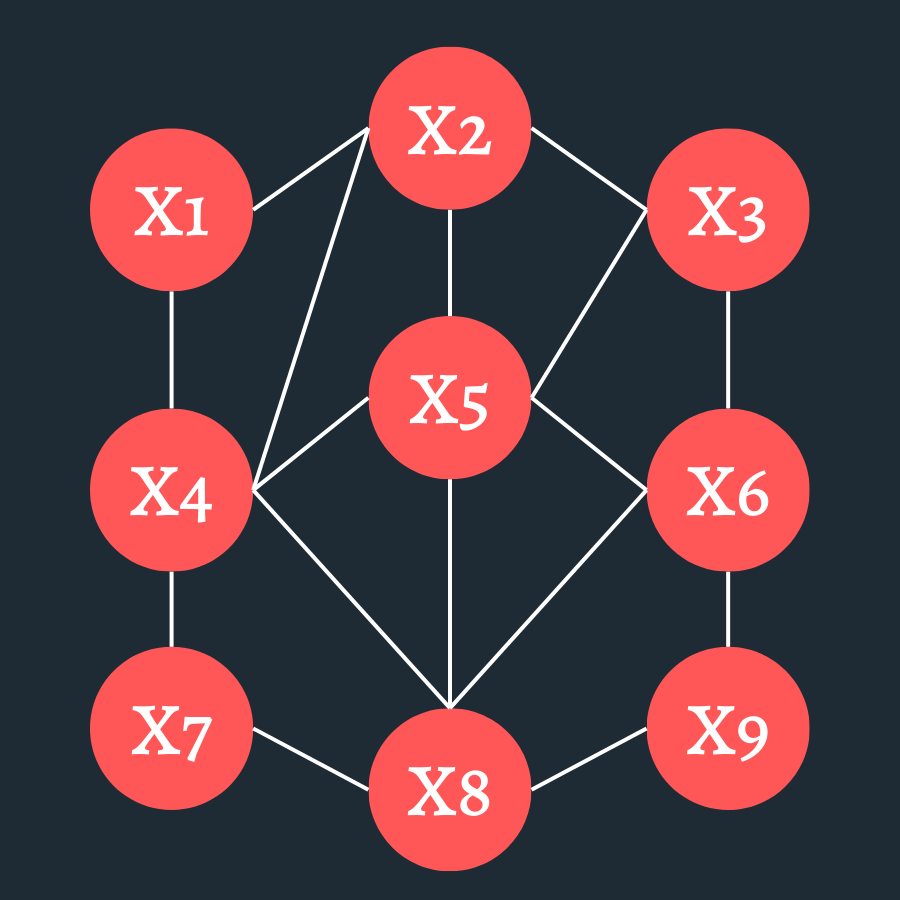
\includegraphics[scale = .3]{assets/imagenes/grafo.png}
    \end{center}
    
    $(x_1 , x_2 , x_4)$ representan los vértices para la primera cláusula $((x_1 \vee \bar{x}_2 \vee x_3))$.
    $(x_5 , x_6 , x_8)$ representan los vértices para la segunda cláusula $((x_2 \vee \bar{x}_3 \vee x_4))$.
    $(x_7 , x_9 , x_3)$ representan los vértices para la tercera cláusula $((\bar{x}_1 \vee x_2 \vee \bar{x}_4))$.
    Las aristas entre $(x_1 , x_2 , x_4)$; $(x_5 , x_6 , x_8)$; y $(x_7 , x_9 , x_3)$ forman los triángulos de cláusula.
    Las aristas que conectan estos triángulos representan las relaciones entre las variables y las cláusulas.

    \item Verificación de la Coloración 
    
    Si podemos asignar colores a este gráfico de tal manera que los vértices conectados directamente 
    no compartan el mismo color, entonces la instancia original de 3SAT es satisfactoria. Si no podemos 
    encontrar tal asignación de colores, entonces la instancia de 3SAT no es satisfactoria.
\end{enumerate}


% ------------------------------------------------------------------------------\
% -----------------------------------------------------------------------------\
\subsection{\textcolor{Contraste4}{Técnicas de demostración}}
% ------------------------------------------------------------------------------\
% -----------------------------------------------------------------------------\
\subsubsection*{\textcolor{Contraste3}{Reducción}}

Se utiliza una reducción polinomial de 3SAT a 3-coloración. Esta reducción demuestra que 3-coloración 
es al menos tan difícil como 3SAT, ya que si se pudiera resolver 3-coloración en tiempo polinomial,
también se podría resolver 3SAT en tiempo polinomial.

\subsubsection*{\textcolor{Contraste3}{Diseño de componentes}}

Se utilizan triángulos como componentes básicos para construir la instancia de 3-coloración a partir de la 
instancia de 3SAT. Los triángulos permiten representar las variables y las cláusulas de una manera que se 
puede colorear de manera válida si y solo si la instancia de 3SAT es satisfactible.

% ------------------------------------------------------------------------------\
% -----------------------------------------------------------------------------\
\subsection{\textcolor{Contraste4}{Aplicación}}
% ------------------------------------------------------------------------------\
% -----------------------------------------------------------------------------\

Imaginemos que una universidad que necesita programar exámenes finales para diferentes 
materias. Algunos estudiantes están inscritos en múltiples cursos, por lo que la 
universidad quiere asegurarse de que no haya exámenes encimados para los estudiantes.\\ 

\textbf{Problema de 3-Coloración:} Cada curso se representa como un vértice en una gráfica. 
Si dos cursos tienen estudiantes en común, se conectan con una arista. El objetivo es 
colorear la gráfica (es decir, programar los exámenes) de tal manera que ningún par de 
vértices adyacentes (cursos con estudiantes en común) tengan el mismo color 
(exámenes en el mismo día).

\subsubsection*{\textcolor{Contraste3}{Solución}}

\begin{myitemize}
    \item Se crea un gráfica donde cada vértice representa un curso.
    \item Se añade una arista entre dos vértices si los cursos correspondientes tienen estudiantes en común.
    \item Se colorean los vértices de tal manera que no haya dos vértices adyacentes con el mismo color.
    \item Cada color representa un día diferente de exámenes.
\end{myitemize}

\subsubsection*{\textcolor{Contraste3}{Ejemplo}}

Tenemos 7 materias: ICC, Modelado, Bases de datos, Complejidad, IA, Probabilidad, Autómatas \\ 

\begin{myitemize}
    \item ICC y Modelado comparten estudiantes.
    \item ICC y Bases de datos comparten estudiantes.
    \item ICC y Autómatas comparten estudiantes.
    \item Modelado y Autómatas comparten estudiantes.
    \item Bases de datos y Complejidad comparten estudiantes.
    \item Complejidad y IA comparten estudiantes.
    \item IA y Probabilidad comparten estudiantes.
\end{myitemize}

Se asigna un color (día de examen) a cada curso de tal manera que ningún estudiante tenga dos exámenes el mismo día.\\ 


\textbf{Resultado:}
\begin{itemize}
    \item[] Día 1 (Color 1): ICC, Bases de datos, IA
    \item[] Día 2 (Color 2): Modelado, Autómatas
    \item[] Día 3 (Color 3): Complejidad, Probabilidad
\end{itemize}

\noindent Este método asegura que todos los estudiantes puedan asistir a sus exámenes sin conflictos de horario.